\chapter{Mini Problems}

\section{Greatest Common Divisor}
\begin{exercise}
    Write a function to calculate the GCD of two integers.
    \begin{example}
        \label{ex:gcd:example1}
        \hfill \\
        Given $35$ and $28$ the function returns $7$.
    \end{example}
    
    \begin{example}
        \label{ex:gcd:example2}
        \hfill \\
        Given $15$ and $8$ the function returns $1$.
    \end{example}

    \end{exercise}

\subsection{\CC Brute-force}
The GCD of two numbers $x$ and $y$ is defined as the largest integer that divides both $x$ and $y$. A simple and inefficient solution would simply loop over all numbers from the smallest between $x$ and $y$ and would stop as soon as we find one that divides both. We are guaranteed to find such a nuber as the number $1$ will happily divide any number. This solution is shown in Listing \ref{list:gcd_bruteforce}.

\lstinputlisting[language=c++, caption={Brute-force, linear time solution.},label=list:gcd_bruteforce]{test/mini_problems/gcd/gcd_bruteforce.cpp}

\subsection{Log-time solution. Euclidean Algorithm}
A much faster solution can be achieved by using the Euclidean algorithm for the GCD.
This algorithm is based on the principle that the greatest common divisor of two numbers $x$ and $y$ does not change if the larger number is replaced by the reminder of the integral division between $x$ and $y$.

For example, $21$ is the GCD of $252$ and $105$ (as $252 = 21 \times 12$ and $105 = 21 \times 5$), and the same number $21$ is also the GCD of $105$ and $252 \mod 105 = 42$.
Since this replacement reduces the larger of the two numbers, repeating this process gives successively smaller pairs of numbers until we reach a point where the smallest numbers divides the largest and therefore the reminder is zero (in the worst case the smallest becomes $1$). 

It was proven by Gabriel Lamé in 1844 that this algorithm always terminates in less steps than five times the number of digits of the smaller number (in base 10) making this algorithm extremely efficient as the number of digits grows logaritmically compared the number it represents.

Listing \ref{list:gcd_euclide} shows a recursive implementation of this algorithm while Listing \ref{list:gcd_euclide_iterative} shows an iterative one. 

\lstinputlisting[language=c++, caption={Euclide algorithm, recursive implementation.},label=list:gcd_euclide]{test/mini_problems/gcd/gcd_euclide.cpp}

\lstinputlisting[language=c++, caption={Euclide algorithm, iterative implementation.},label=list:gcd_euclide_iterative]{test/mini_problems/gcd/gcd_euclide_iterative.cpp}

\subsection{\CC Compile-time}
It is quite common to see specific requirements on the compile implementation of the GCD algorithm. Therefore in this section we will see how we can calculate the GCD in \CC at compile time. 

Before C++-11 the only way to do compile time computation was by using templates. In order to calculate GCD using templates we will use a structure with two integral template parameters that we will manipulate in a \inline{static const} variable. An implementation of this idea is shown in \ref{list:gcd_euclide_precpp11}.

\lstinputlisting[language=c++, caption={Pre C++11, compile-time template based solution.},label=list:gcd_euclide_precpp11]{test/mini_problems/gcd/gcd_euclide_pre_cpp11.cpp}

The code works by have a template class with two integral template parameters and a partial specialization that is used to terminate the recursion which is triggered whenever we request the static field \inline{::gcd}.

C++-11 introduces \inline{constexpr} function that can be used to specify function that can be run at compile-time. In C++-11 there are quite some limitation in what statements and operations we can do in a \inline{constexpr} context: for instance we can only have one return statement. Most of these contraints are related in the subsequent versions of the standard. A \inline{constexpr} recursive solution that works in C++-11 is shown in Listing \ref{list:gcd_euclide_cpp11}.

\lstinputlisting[language=c++, caption={C++11 \inline{constexpr} based solution.},label=list:gcd_euclide_cpp11]{test/mini_problems/gcd/gcd_euclide_cpp11.cpp}

Notice that, from C++-14 we can decorate Listing \ref{list:gcd_euclide_iterative} with \inline{constexpr} so that it can be used in compile-time computation.



%%%%%%%%%%%%%%%%%%%%%%%%%%%%%%%%%%%%%%%%%%%%%%%%%%%%%%%%%%%

\section{Maximum Depth of N-ary Tree}
\begin{exercise}
   Given a N-ary tree, return its depth which is defined as the length of the longest path from the tree's root to any of its leaves.
    \begin{example}
        \label{ex:nary-treedepth:example1}
        \hfill \\
        Given the tree depicted in Figure \ref{fig:longest_consecutive_sequence:example1} the function returns $3$ (path from node $1$ to node $12$).
    \end{example}
    
    \begin{example}
        \label{ex:nary-treedepth:example2}
        \hfill \\
        Given the tree depicted in Figure \ref{fig:longest_consecutive_sequence:example2} the function returns $6$ (path from node $1$ to node $40$).
    \end{example}
    \end{exercise}
 
 
\begin{figure}
	\centering
	\begin{subfigure}[]{0.45\textwidth}
		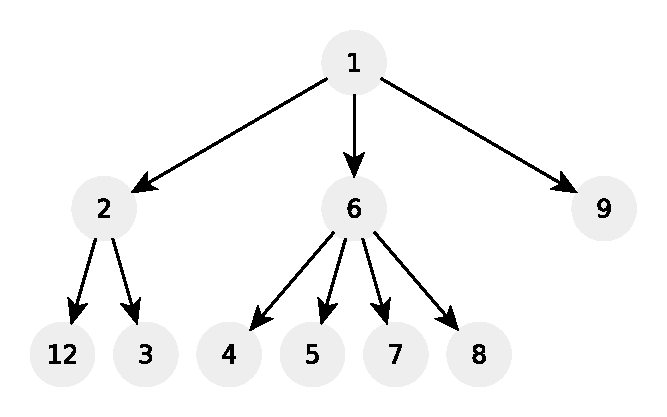
\includegraphics[width=1\linewidth]{sources/mini_problems/n-ary-tree-depth/images/example1}
		\caption{Input tree for Example \ref{ex:nary-treedepth:example1}.}
		\label{fig:longest_consecutive_sequence:example1}
	 \end{subfigure}
	\hfill
	\begin{subfigure}[]{0.45\textwidth}
		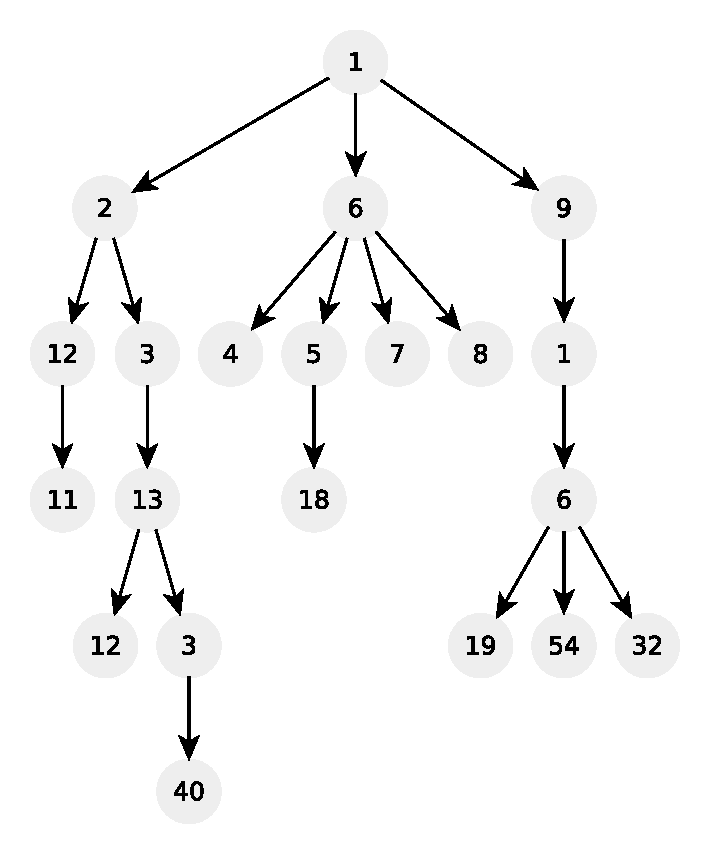
\includegraphics[width=1\linewidth]{sources/mini_problems/n-ary-tree-depth/images/example2}
		\caption{Input tree for Example \ref{ex:nary-treedepth:example2}.}
		\label{fig:longest_consecutive_sequence:example1}
	 \end{subfigure}
	 \caption[]{}
	  \label{}
\end{figure}
    
\subsection{Discussion}
    This is a classical problem, mostly asked during phone screening due to its simplicity. 
    What the problem, in other words, is asking us to do, is to return the maximum level of any of the tree's nodes.
    The level of a node is the number of its ancestors plus one. 
    Therefore to solve this problem, all we have to do is to visit the tree and keep track of the number of ancestors which is equivalent to the number of steps down the tree we took.
    We know that the root has $0$ ancestors and therefore, we know that each of its children will have $1$ ancestor (the root itself) and that any of its grandchildren will have $2$ ancestors and so on.
    
    Visiting a tree can be equally easily done recursively and iteratively as shown in Sections \ref{} and \ref{}, respectively.
 
    For the reminder of the discussion, we will define the root of a tree to be a pointer to the \inline{Node} structure defined in Listing \ref{list:n-arytreedepth:nodedef}.
 
    \begin{lstlisting}[language=c++, caption={Node definition.},label=list:n-arytreedepth:nodedef]]{
class Node {
public:
    int val;
    vector<Node*> children;

    Node() {}

    Node(int _val) {
        val = _val;
    }

    Node(int _val, vector<Node*> _children) {
        val = _val;
        children = _children;
    }
};            
    \end{lstlisting} 
    

\subsection{Recursive solution}
The recursive solution has the advantage of being shorter in terms of lines of code and in our opinion more elegant. It could, however, underperform the iterative solution if the compiler is not able to optimize the code properly or lead to out of memory errors if the tree depth goes over a certain value because at any given time, we keep in the stack a number of activation records that is equal to the level of the node we are visiting.

Listing \ref{list:n-ary-treedepth_recursive}  shows an implementation of this approach and has a linear time and space (considering the space occupied by the activation records) in the number of nodes of the tree.

\lstinputlisting[language=c++, caption={Recursive solution.},label=list:n-ary-treedepth_recursive]{test/mini_problems/n-ary-treedepth/n-ary-treedepth_recursive.cpp}

\subsection{Iterative Solution}
The same idea can be implemented iteratively as shown in Listing \ref{list:n-ary-treedepth_iterative} where we use a stack to keep track of the nodes \textbf{and their level}. Whenever we visit a node, we compare its level with the maximum found so far, then we remove it from the stack and insert all of its children in the stack with a level value increased by one. 

\lstinputlisting[language=c++, caption={Iterative solution.},label=list:n-ary-treedepth_iterative]{test/mini_problems/n-ary-treedepth/n-ary-treedepth_iterative.cpp}


%%%%%%%%%%%%%%%%%%%%%%%%%%%%%%%%%%%%%%%%%%%%%%%%%%%%%%%%%%%

\section{Assigning cookies \faCookie}
\begin{exercise}
    You are the parent of $n$ children and you want to make them happy by giving them a cookies (real ones  \faCookieBite, not HTTP cookie). 
    However you know that too many cookied are not good for them and therefore you settle for a rule that each child can at most get one cookie.
    Giving cookies to your children is not easy as they are special and each child $i$ has an integer greed factor $g[i]$ associated,
    which is the minimum size of a cookie that the child $i$ will be content with; 
    You have at your disposal a number $m$ of cookies, and each cookie $j$ has an integer size $s[j]$.
    You can give cookie number $i$ to child number $i$ if and only if $s[j] \ge g[i]$. When a child has a cookie assigned is content.
    
    Write a function that given a list  ($G$) of $n$ greed values and a list ($C$) of  $m$ cookie sizes determines the maximum possible of children you can make content.
     
    \begin{example}
        \label{ex:nary-treedepth:example1}
        \hfill \\
        Given $G=\{1,2,3\}$ and  $=\{1,1\}$ the function returns $1$. Despite having two cookies we can only make one child happy because we do not have cookies big enough for children number $2$ and $3$.
    \end{example}
    
    \begin{example}
        \label{ex:nary-treedepth:example2}
        \hfill \\
        Given $G=\{1,3\}$ and  $=\{1,4\}$ the function returns $2$. We can give the first cookie to the first child and the second cookie to the second child.
    \end{example}


    \begin{example}
        \label{ex:nary-treedepth:example3}
        \hfill \\
        Given $G=\{1,2,3\}$ and  $=\{1,1,3\}$ the function returns $2$. We can give the first cookie to the first child and the the third cookie to the second child The second cookie remains unassigned and the third child without cookie assigned.
    \end{example}
    \end{exercise}
 

\subsection{Discussion}
Let's start by noticing that despite what shown in the Exmaples the input lists are not guaranteed to be sorted and that, sorting actually makes solving this problem much easier.
The idea is that we have to find a way to assign to each children the smallest cookie possible that has size higher or equal to his greed. If the input array is not sorted then for each greed value we are forced to search $S$ entirely for a suitable cookie. 
If on the other hand both $G$ and $S$ are sorted then, we can try to accomodate children by increasing greed and keep track and assign progressively larger cookies to them. 
If a children with greed $i$ can be assigned cookie number $j$, then we can try to assign to child number $i+1$ cookie number $j+1$. If that does not work then we can try with cookie number $j+2$ and so on.
When we cannot assign a cookie $j$ to a certain child $i$, cookie $j$ will be unused, but that is not an issue because there is no way we can assign cookie $j$ to any other children because the greed values for children $i+1, i+2, \ldots$  will all be greater than the gree of child $i$.

Therefore in order to solve this problem we can:
\begin{itemize}
    \item sort $G$;
    \item sort $S$;
    \item use two pointers to keep track of the current child and current cookie
    \item process one child a the time until we ran out of children or cookies
    \item if the current cookie size is greater than the current child greed then we can advance both pointers
    \item otherwise we can only hope the next cookie will be assignable and therefore only advance the cookie pointer.
\end{itemize}

An implementation of this idea is shown in Listing \ref{list:assign_cookies_sorting}. Its time complexity is $O(nlog(n))$ while its the space complexity is $O(1)$.


\lstinputlisting[language=c++, caption={Solution using sorting.},label=list:assign_cookies_sorting]{test/mini_problems/assign_cookies/assign_cookies_sorting.cpp}


%%%%%%%%%%%%%%%%%%%%%%%%%%%%%%%%%%%%%%%%%%%%%%%%%%%%%%%%%%%

\section{Maximize Sum Of Array After K Negations}
\begin{exercise}
    Given an integer array $nums$ and an integer $k$, modify the array in the following way: choose an index $i$ and replace $nums[i]$ with $-nums[i]$.
    
    You should apply this process \textbf{exactly} $k$ times. You may choose the same index $i$ multiple times.
    
    Return the largest possible sum of all the elements of $nums$ at end of this process.     
    \begin{example}
        \label{ex:nary-treedepth:example1}
        \hfill \\
        Given $nums=\{4,2,3\}$ and $k=1$ the function returns $5$. We can choose index $1$ and turn the $2$ into $-2$. At the end we will be left with $nums=\{4,-2,3\}$ which totals to $4-2+3=5$.
    \end{example}
    
    \begin{example}
        \label{ex:nary-treedepth:example2}
        \hfill \\
        Given $nums=\{3,-1,0,2\}$ and $k=3$ the function returns $6$. We can choose 
    \end{example}


    \end{exercise}
 

\subsection{Discussion}
One easy way of solving this problem relies on the fact that all we have to do is to apply the change sign change always on the smallest number of the array.
The intuition behind it is that we should aim at first changing the sign of all the negative numbers first and among them we should prioritize the smallest ones: the number with the largest absolute value and negative sign. Changing the sign of those number will bring the best increase in the overall sum of the array.

If after having changed all negatives into positive we are left with more moved to make then we still have to change the sign of the smallest number in the array as many times as necessary.
This causes the smallest number of the array to switch sign back and forth until $k=0$ (this step can be optimized by noticing that if the number of moves left is even then the final valud of the smallest number in the array is not going to change, otherwise, it will be negative.We can reach this conclusion without having to actually perform the sign switch). 

To always keep track of the smallest number we can use a \inline{std::priority_queue} as shown in Listing \ref{}.

\lstinputlisting[language=c++, caption={Solution using sorting.},label=list:assign_cookies_sorting]{test/mini_problems/max_sum_array_after_k_negations/max_sum_array_after_k_negotiation_priority_queue.cpp}

The code works by applying the $k$ modifications always to the smallest element of the queue. At the end of the process we simply sum every element in the queue to obtain the answer. The complexity of this approach is $O(klog(n) + nlog(n))$ in time and $O(1)$ in space.

